\section{Durchführung}

\noindent
Der Versuchsaufbau ist in Abbildung \ref{fig:aufbau} dargestellt.
Teil des Aufbaus sind der Sinusgenerator, die Resonatoren sowie das Oszilloskop.

\begin{figure}
  \centering
  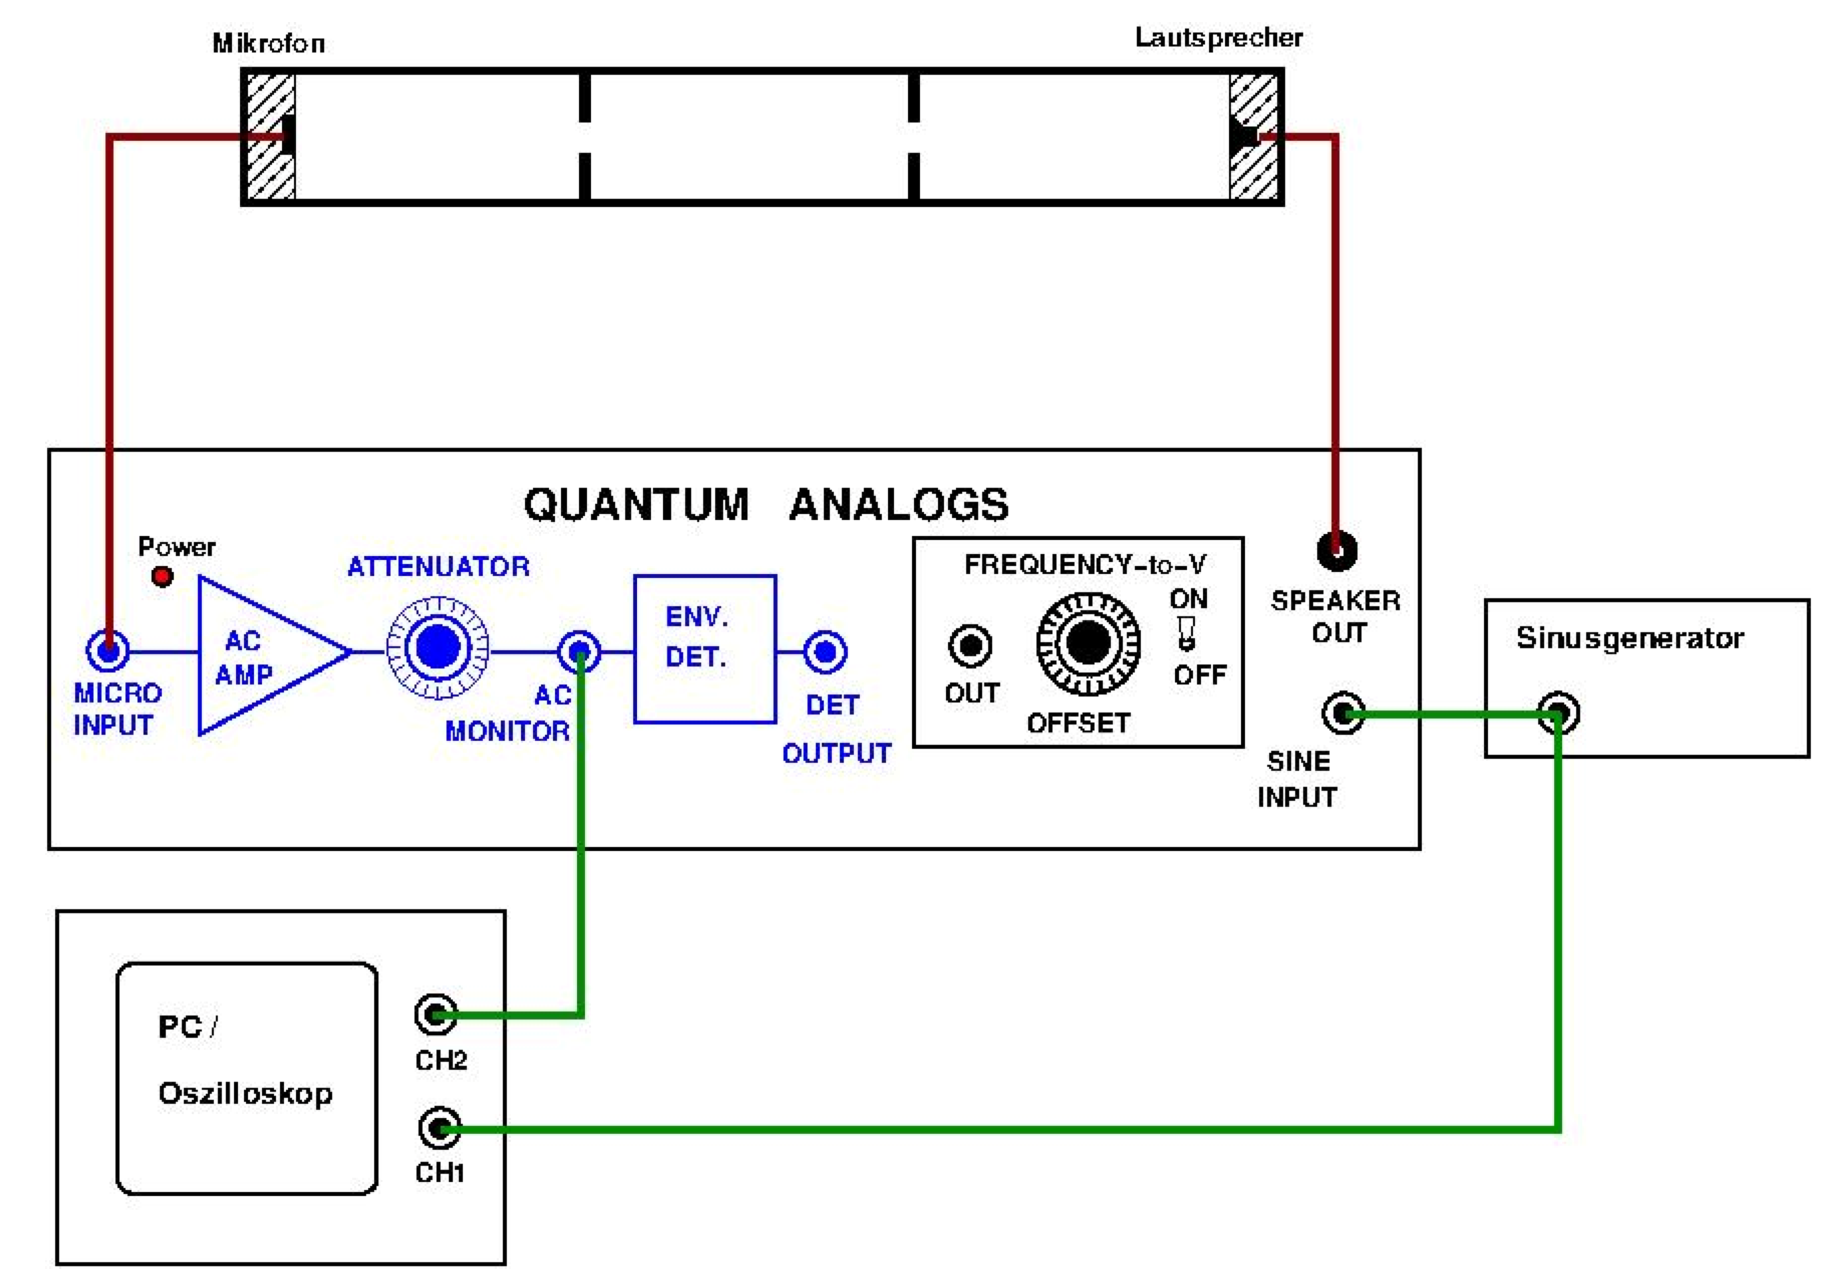
\includegraphics[width=0.75\textwidth]{V23_aufbau.png}
  \caption{Versuchsaufbau \cite{V23}}
  \label{fig:aufbau}
\end{figure}


\subsection{Das Wasserstoffatom}
\label{Wasserstoffatom}
\noindent
Der Kugelresonator mit dem das Wasserstoffatom simuliert wird besteht aus zwei zusammengesetzten Halbkugeln mit Lautsprecher und Mikrofon im Inneren.
Bei einem Winkel von $\alpha=$180° liegen dabei Lautsprecher und Mirkrofon genau gegenüber.
Zunächst wird bei einem Winkel von 180° ein hochaufgelöstes Frequenzspektrum mit 5Hz-Schritten bei $60\frac{\text{ms}}{\text{Schritt}}$ mithilfe des PCs aufgenommen.

\noindent
Danach werden die Resonanzfrequenzen untersucht, indem die Frequenz händisch am Sinusgenerator von 100Hz bis 10kHz abgefahren wird und die Amplitude am Oszillokop beobachtet
, die Pieks notiert und die Phasenverschiebung bestimmt wird.

\noindent
Für vier Resonanzfrequenzen werden nun Frequenzspektren aufgenommen, wobei der Drehwinkel von 0° bis 180° in 10° Schritten variiert wird.

\noindent
Nun wird ein 3mm Ring zwischen die Halbkugeln eingesetzt.
Bei einem Winkel von 180° wird die Aufspaltung der Resonanzfrequenz um 2,3kHz vermessen.
Die Messung wird für den 6mm Ring und der Kombination beider Ringe (9mm) wiederholt.

\noindent
Zuletzt wird die Winkelabhängkeit der Resonanzfrequenz um 2,3kHz mit dem 9mm Zwischenring vermessen.
Dafür wird von einem Winkel von 0° bis 180° in 10° Schritten gemessen.

\subsection{Das Wasserstoffmolekül}
\noindent
Für das Wasserstoffmolekül wird ein weiterer Kugelresonator zwischen Lautsprecher und Mikrofon gesetzt.

\noindent
Zuerst wird ein hochaufgelöstes Frequenzspektrum bei der Resonanz von 2,3kHz von 2,2kHz bis 2,5kHz mit 1Hz-Schritten bei $75\frac{\text{ms}}{\text{Schritt}}$ aufgenommen.
Dabei werden 10mm, 15mm und 20mm Blenden zwischen die Kugelresonatoren eingesetzt.

\noindent
Mit der 15mm Blende wird nun die Winkelabhängigkeit gemessen.
Dazu wird das Frequenzspektrum um 2,3kHz von 0° bis 180° in 10° Schritten aufgenommen.

\subsection{Der eindimensionale Festkörper}
\label{fkp}

\noindent
Für zwei bis zehn Zylinder wird nacheinander das Frequenzspektrum von 0,1kHz bis 12kHz mit 5Hz-Schritten bei $50\frac{\text{ms}}{\text{Schritt}}$ aufgenommen.
Zwischen den 50mm Zylindern befinden sich dabei 16mm Blenden.

\noindent
Der Vorgang wird für zwei, vier und zehn 50mm Zylinder wiederholt, wobei die 16mm Blenden mit 10mm und 13mm Blenden ausgetauscht werden.

\noindent
Ausgehend von zehn 50mm Zylindern mit 16mm Blenden wird ein Zylinder mit einem 75mm, 37,5mm und 62,5mm Zylinder ausgetauscht und das Spektrum wird aufgenommen.

\noindent
Anschließend wird das Spektrum von zehn abwechselnd 50mm und 75mm Zylindern aufgenommen, wobei je 16mm zwischengesetzt wurden.

\noindent
Zuletzt werden acht 75mm Zylinder mit abwechselnd 13mm und 16mm Blenden aneinandergereiht.



